\documentclass[french]{amu_these}

\begin{document}

										
	\chead{}
\pdfbookmark[0]{Page de titre}{titre}
\thispagestyle{empty}
\newgeometry{margin=2em}
% \newgeometry{left=3em,right=2em,top=2em,bottom=2em} %% marge pour la reliure en cas d'exemplaire imprimé

\begin{center}
	\begin{minipage}[c]{.5\linewidth}
		\raggedright
\includegraphics[height=7em]{logo_amu_excellence}
	\end{minipage}\hfill
	\begin{minipage}[c]{.5\linewidth}
		%\raggedleft\includegraphics[height=7em]{example-image-b} %% logo cotutelle
	\end{minipage}\hfill
\end{center}

\vspace{1em}

\begin{center}
	\begin{minipage}[c]{.63\linewidth}
		\dhorline{\textwidth}{4pt}
	\end{minipage}\hfill
	\begin{minipage}[c]{.35\linewidth}
		\raggedleft\titl{NNT/NL : 2020AIXM0001/001ED000}
		% renseigner votre numéro national de thèse (NNT) et le numéro local (NL)
		% ils sont indiqués sur la page d'informations administratives de votre espace de dépôt dans le guichet de dépôt légal des thèses AMU lorque votre date de soutenance est renseignée par votre service de scolarité
		% https://depot-theses.univ-amu.fr/
	\end{minipage}\hfill
\end{center}

%\vspace{1em}

\doublespacing
\begin{flushleft}
    \titb{\HUGE\textcolor{cyanamu}{THÈSE DE DOCTORAT}}\\
	\titl{\Large Soutenue à Aix-Marseille Université}\\
	%\titl{\Large dans le cadre d'une cotutelle avec }\\
	\titl{\Large le 10 janvier 2020 par}\\
\end{flushleft}
\vspace{2em}
\begin{center}
	\titsb{\Huge Prénom NOM}\\
    \vspace{1em}
	\titm{\LARGE Titre de la thèse:\\ sous-titre de la thèse}\\
\end{center}
\singlespacing

\vspace{4em}

\begin{center}
	\begin{minipage}[t]{.45\linewidth}
    	    \vspace{.5em}
        	\titb{Discipline}
        	
        	\titl{renseigner la discipline du doctorat (\hyperref[chap:doctorats]{Annexe A})}
        	
    	    \vspace{1em}
        	\titb{Spécialité}
        	
        	\titl{renseigner la spécialité du doctorat (\hyperref[chap:doctorats]{Annexe A})}
        	
    	    \vspace{2em}
        	\titb{École doctorale}
        	
        	\titl{renseigner l'école doctorale (\hyperref[chap:doctorats]{Annexe A})}
        	
    	    \vspace{1em}
        	\titb{Laboratoire/Partenaires de recherche}
        	
        	\titl{renseigner les partenaires institutionnels
        	
        	et les partenaires privés
        	
        	un partenaire par ligne
        	}
	\end{minipage}\hfill
	\begin{minipage}[t]{.03\linewidth}
	    \dvertline{4pt}{-16em}
	\end{minipage}\hfill
	\begin{minipage}[t]{.52\linewidth}
	    \vspace{.5em}
    	\titb{\small Composition du jury}

	    \vspace{1em}
    	\titel{
        \begin{tabular}{p{12em} p{9.5em}}
        	Prénom NOM & Rapporteur·e \\
        	Affiliation \\
        	\\
        	Prénom NOM & Rapporteur·e \\
        	Affiliation \\
            \\
            Prénom NOM & Examinateur·rice \\
        	Affiliation \\
            \\
        	Prénom NOM & Président·e du jury \\
        	Affiliation \\
            \\
        	Prénom NOM & Directeur·rice de thèse \\
        	Affiliation \\
        \end{tabular}
        }
	\end{minipage}\hfill
\end{center}       

\vspace{2em}

\begin{center} %% logos partenaires
	\begin{minipage}[c]{.25\linewidth}
		\centering\includegraphics[height=5em]{example-image-a} 
	\end{minipage}\hfill
	\begin{minipage}[c]{.25\linewidth}
		\centering\includegraphics[height=5em]{example-image-b}
	\end{minipage}\hfill
	\begin{minipage}[c]{.25\linewidth}
		\centering\includegraphics[height=5em]{example-image-c} 
	\end{minipage}\hfill
	\begin{minipage}[c]{.25\linewidth}
		\centering\includegraphics[height=5em]{example-image-c}
	\end{minipage}\hfill
\end{center}

\restoregeometry				%% page de titre
										
	\newpage
\chapter*{Affidavit}					
\addcontentsline{toc}{chapter}{Affidavit}
\thispagestyle{empty}
\iffalse % Déclaration sur l'honneur pour une thèse en français (inverser les \if pour une thèse en anglais)
    Je soussigné, [Prénom Nom], %% Prénom et Nom de l'auteur %%
    déclare par la présente que le travail présenté dans ce manuscrit est mon propre travail, réalisé sous la direction scientifique de [Prénom Nom], % Prénom et Nom du directeur de thèse et s’il y a lieu du co-directeur de thèse
    dans le respect des principes d’honnêteté, d'intégrité et de responsabilité inhérents à la mission de recherche. Les travaux de recherche et la rédaction de ce manuscrit ont été réalisés dans le respect à la fois de la charte nationale de déontologie des métiers de la recherche et de la charte d’Aix-Marseille Université relative à la lutte contre le plagiat.
    
    Ce travail n'a pas été précédemment soumis en France ou à l'étranger dans une version identique ou similaire à un organisme examinateur.\\
    
    Fait à [ville] le [date]
    
    \begin{flushright}\includegraphics[width=120px,height=40px]{example-image-a}\end{flushright}% signature
\fi

\iftrue % Affidavit of Honour for english thesis (invert the \if for an English thesis)
    I, undersigned, Felipe Torres Figueroa, %% First Name and Surname of the PhD student
    hereby declare that the work presented in this manuscript is my own work, carried out under the scientific direction
    of Stephane Ayache, Ronan Sicre and Yannis Avrithis; %% First Name and Surname of the thesis director and if applicable of the co-thesis director
    in accordance with the principles of honesty, integrity and responsibility inherent to the research mission. The research work and the writing of this manuscript have been carried out in compliance with both the french national charter for Research Integrity and the Aix-Marseille University charter on the fight against plagiarism.
    
    This work has not been submitted previously either in this country or in another country in the same or in a similar version to any other examination body.\\
    
    Marseille, June-10$^{th}$, 2024
    
    \begin{flushright}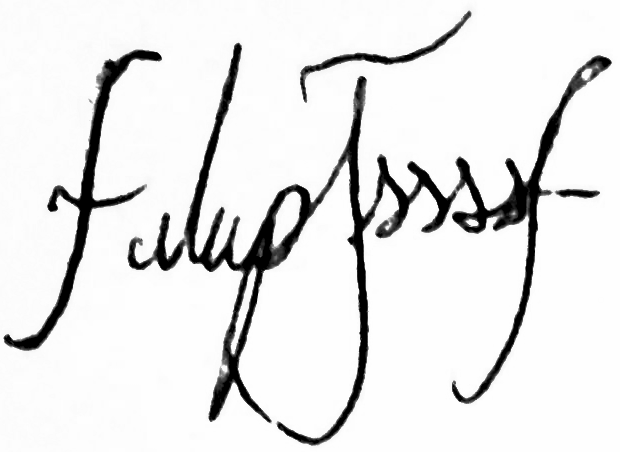
\includegraphics[width=120px,height=40px]{tex_open/support/corrected}\end{flushright} % signature
\fi

~\vfill
\begin{center}
	\begin{minipage}[c]{0.25\linewidth}
		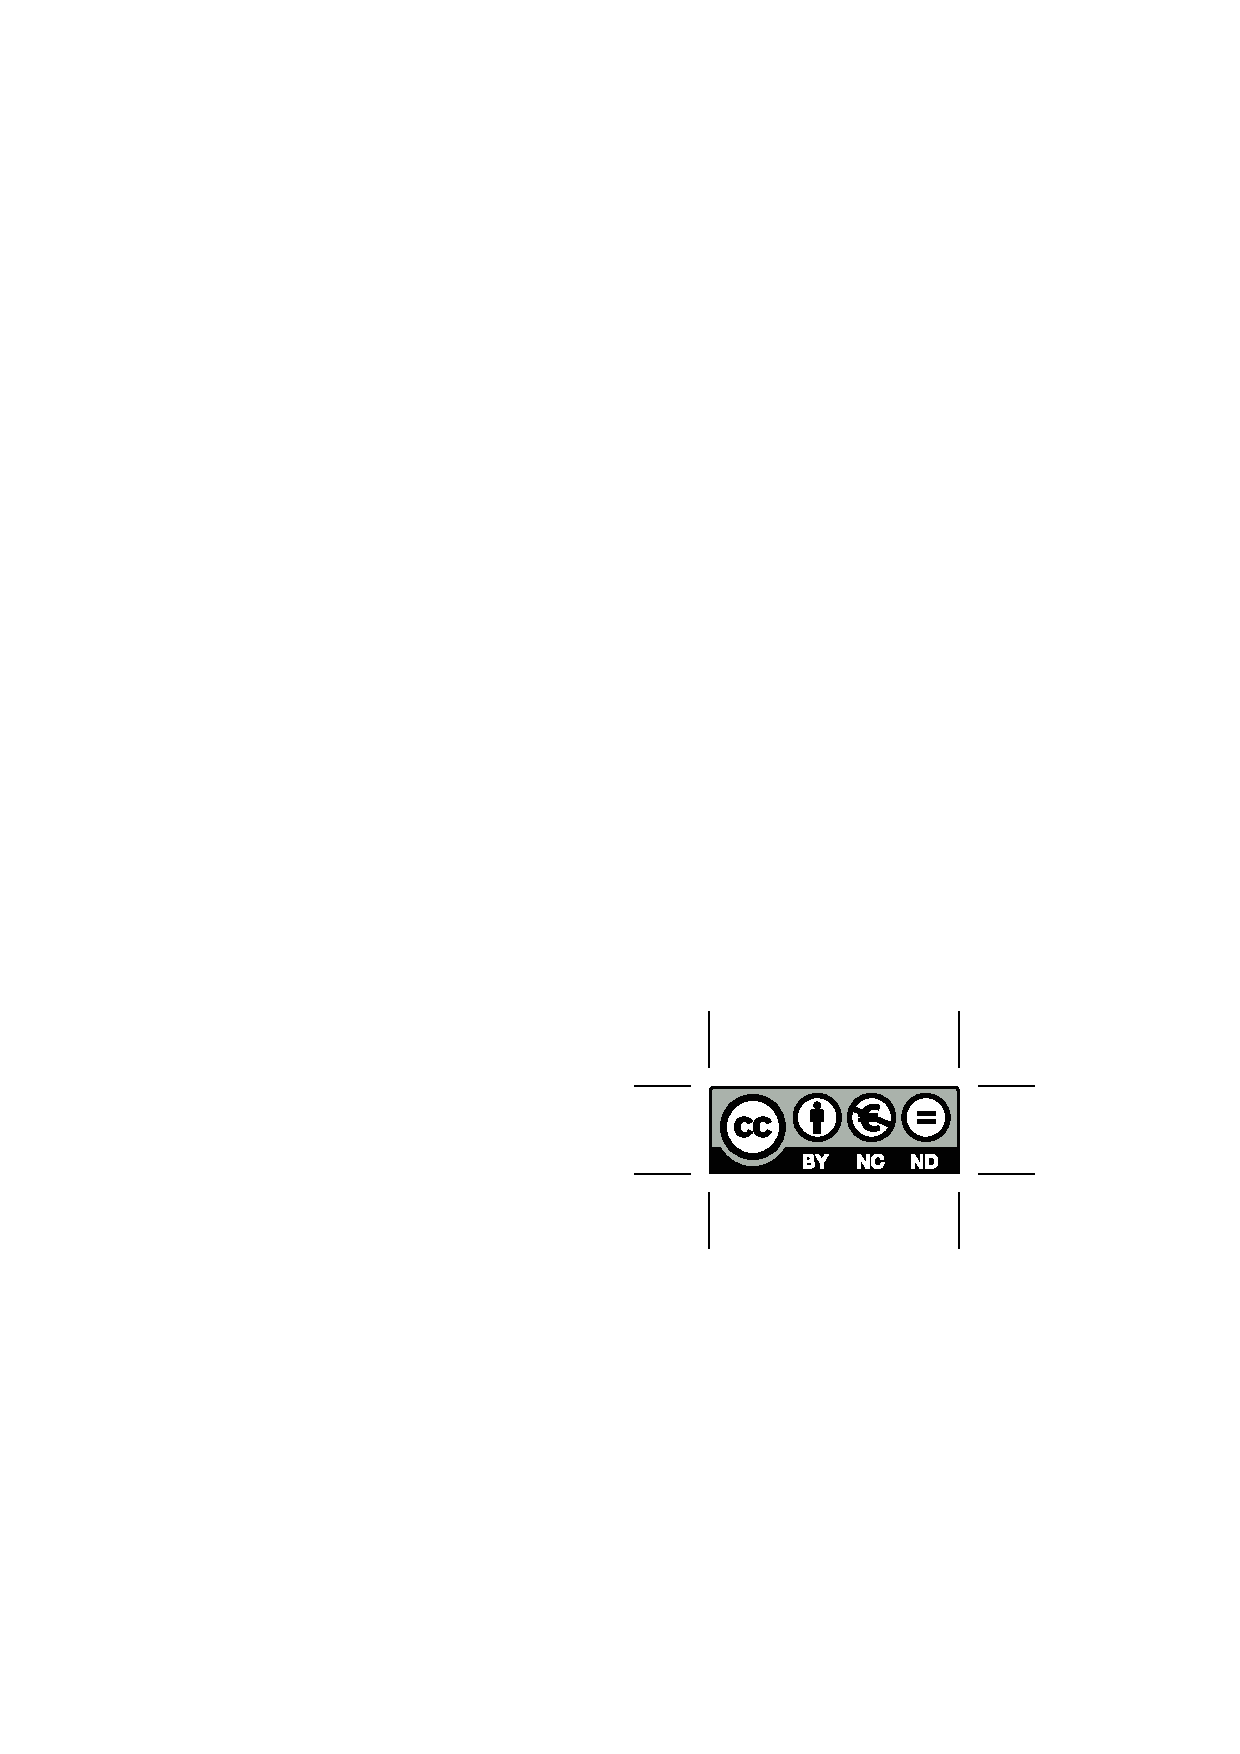
\includegraphics[height=35px]{by-nc-nd-eu}
	\end{minipage}\hfill
\end{center}

Cette \oe{}uvre est mise à disposition selon les termes de la \href{https://creativecommons.org/licenses/by-nc-nd/4.0/deed.fr}{Licence Creative Commons Attribution - Pas d’Utilisation Commerciale - Pas de Modification 4.0 International}. % consultez les conditions de la licence cc by-nc-nd, vous pouvez appliquer une licence moins restrictive, cc by-nc-sa par exemple
				%% affidavit et licence

	\newpage
\chapter*{Liste de publications et participation aux conférences}
\addcontentsline{toc}{chapter}{Liste de publications et participation aux conférences}
\subsection*{Liste des publications réalisées dans le cadre du projet de thèse:}
\begin{enumerate}
    \item Opti-CAM: Optimizing saliency maps for interpretability. (Pattern Recognition, under revision)
    \item CA-Stream: Attention-based pooling for interpretable image recognition. (-)
    \item A Learning Paradogm for Interpretable Gradients. (VISAPP 2024)
    \item The concept of Zero Information in Explainable AI
\end{enumerate}


\subsection*{Participation aux conférences et écoles d’été au cours de la période de thèse:}
\begin{enumerate}
\item ELLIS Summer School on Large-Scale AI for Research and Industry. Modène, Italie.
\end{enumerate}
			%% liste de publications et participation aux conférences

	%--------------------------------------------------------------------------------------------------
\chapter*{Résumé}
\addcontentsline{toc}{chapter}{Résumé}
Les applications de vision par ordinateur utilisant les technologies de l'intelligence artificielle 
ont connu une évolution remarquable au cours de la dernière décennie. Les développements actuels en 
vision par ordinateur sont le résultat direct d'une meilleure utilisation du matériel, permettant 
la construction de modèles capables d'effectuer des tâches plus complexes au fil du temps. En ce 
qui concerne la reconnaissance d'images en particulier, les réseaux neuronaux convolutionnels et 
les transformateurs sont désormais capables d'identifier les images et leurs éléments, ainsi que 
d'attribuer une valeur sémantique à ces derniers, même dans des conditions difficiles.\\

\noindent Avec la diffusion des technologies de l' apprentissage profond au sein de la société, 
une nouvelle exigence a émergé pour ces méthodologies. Puisqu 'elles interagissent désormais et 
affectent directement les vies humaines, il est impératif de comprendre leur fonctionnement et de 
fournir des explications. Pour répondre à ces questions, un nouveau domaine de recherche a vu le 
jour: l 'interprétabilité et l 'IA explicable.\\

\noindent Dans cette thèse, notre objectif est de comprendre et de développer des modèles 
d'interprétabilité pour les modèles de reconnaissance d'images de pointe. Nous présentons et 
expliquons brièvement certains des modèles de reconnaissance d'images les plus performants et 
pertinents pour les Réseaux de Neurones Convolutifs et les Transformers. Ensuite, nous examinons 
les approches actuelles en matière d' interpr\'etabilit\'e conçues pour fournir des explications, 
ainsi que leurs protocoles d' évaluation. Nous faisons des observations sur ces méthodes et 
protocoles d'évaluation, mettant en évidence les difficultés rencontrées et suggérant des idées 
pour surmonter leurs limitations.\\

\paragraph{Opti-CAM} Notre première contribution, s' appuie sur le raisonnement des Cartes d' 
Activation de Classe. En particulier, cette proposition optimise le coefficient de pondération 
requis pour calculer une carte de saillance, générant une représentation qui maximise la 
probabilité spécifique à la classe. Cette carte de saillance offre les meilleurs résultats selon 
les mesures d'interprétabilité, et met en évidence que le contexte est pertinent pour décrire une 
prédiction. De plus, une nouvelle métrique pour compléter l'évaluation de l'interprétabilité est 
dévoilée, remédiant aux lacunes de cette procédure.\\

\paragraph{Cross Attention Stream} Notre deuxième contribution, est un ajout aux modèles actuels de 
reconnaissance d'images, améliorant les mesures d'interprétabilité. Inspiré par des modèles 
novateurs performants tels que les Transformers, nous construisons un flux qui calcule l'interaction 
d'une représentation de classe abstraite avec les caractéristiques profondes des réseaux neuronaux 
convolutionnels. Cette représentation est finalement utilisée pour effectuer la classification. 
Notre flux affiche des améliorations lors de l'évaluation quantitative, tout en préservant les 
performances de reconnaissance à travers différents modèles.\\

\paragraph{Gradient Denoise} Enfin, notre dernière contribution présente un nouveau paradigme d' 
entraînement pour les réseaux neuronaux profonds. De plus, ce paradigme débruite les informations 
de gradient des modèles profonds dans l'espace d'entrée. La représentation de rétropropagation 
guidée de l'image d'entrée est utilisée pour régulariser les modèles lors de leur phase d' 
entraînement. En conséquence, nos modèles entraînés affichent des améliorations pour l' 
évaluation interprétable. Nous appliquons notre paradigme à de petites architectures dans un cadre 
contraint, ouvrant la voie au développement futur dans des ensembles de données à grande échelle, 
ainsi qu'avec des modèles plus complexes.\\

\vspace{0.5cm}
%Keywords: deep learning, image processing, attributions, interpretability
Mots clés: Apprentissage Profond, reconaissance d'image, interpretabilité, explicabilité.
					%% résumé

	%--------------------------------------------------------------------------------------------------
\chapter*{Abstract}
\addcontentsline{toc}{chapter}{Abstract}
Computer Vision applications using Artificial Intelligence technologies have undergone a remarkable 
evolution in the past decade. Current developments in Computer Vision are a direct result of a 
better utilization of hardware, enabling the construction of models capable of performing more 
complex tasks over time. On image recognition in particular, convolutional neural networks and 
transformers are now able to identify images and their elements, as well as assign semantic value 
to them, even in challenging conditions. These models have completely changed the landscape of deep 
learning and image recognition, permeating deep into society with the automatization of many daily 
tasks. Thus, it is no longer a question of \emph{can a model perform 
this task?}, but more a question of \emph{how does this model perform this task?}. To address these 
questions a new research field has emerged: interpretability and explainable AI.\\
\\
%Moreover, progress in this field has paved the way for further developments in complementary fields 
%of Computer Vision: models developed for image recognition are modified to conduct image 
%segmentation and reconstruction.\\

%\noindent The Deep Learning revolution occurred in two stages: first with the reemergence and 
%popularization of convolutional neural networks, and in second place with the 
%introduction of attention based architectures. On one hand, convolutional neural networks were 
%initially hard to train given their complexity and data volume requirements. 
%Still, early proposals showed promise, such as LeNet with the automatic recognition of handwritten 
%digits in the US postal service in the early 1990s. 
%However, in the early years of the last decade these issues were solved with the widespread of 
%large scale visual recognition datasets, as well as with the effective use of Graphics Processing 
%Units for computation. On the other hand, close to the end of this time period a new style of model 
%emerged: the Transformer architecture. This architecture creates an abstract representation of 
%lasses that interacts with every element of an encoding, generating a representation that learns a 
%class representation. Additionally, Transformers can process larger volumes of data, 
%allowing them to be robust to bias and generalize better.\\

%\noindent Convolutional Neural Networks and Transformers 
\noindent In this thesis, our goal is to understand and further develop interpretability models for 
state-of-the-art image recognition models. We introduce and briefly explain some of the most 
relevant high performance image recognition models for both Convolutional Neural Networks 
and Transformers. Then, current interpretability approaches designed to provide 
explanations, as well as their evaluation protocols. We make observations upon 
these methods and evaluation protocols, highlighting difficulties upon them and suggesting ideas 
to address their limitations.\\

\noindent In particular, a novel attribution method is proposed, ensuring that the highlighted 
regions in an image maximize a given class probability. From this method we observe that the 
most important information correlating to a class prediction, is not only found in the object of 
interest. Instead, context conveys salient information too: it is usually spread all over the image. 
Additionally, an addition to existing architectures is introduced, this method enhances predictive 
confidence, boosting interpretability properties of high performing image recognition models. Lastly, we 
propose a learning paradigm, that denoises gradients on the image space, enhancing 
interpretability properties. This final proposition demonstrates improvements on interpretability 
metrics for small datasets and models, while displaying promise for its scaling on to larger 
datasets and architectures.\\

\vspace{0.5cm}
Keywords: Deep Learning, image recognition, interpretability, explainability.

				%% abstract

	\chapter*{Remerciements}
\addcontentsline{toc}{chapter}{Remerciements}
Le modèle de thèse AMU n'existerait pas sans la contribution des doctorants. Nous souhaitons remercier tout particulièrement \href{http://www.theses.fr/2011AIX20720}{Mickaël Bojados}, \href{http://www.theses.fr/2011AIX22111}{Flora Cordoleani} et \href{http://www.theses.fr/2014AIXM4013}{Florian Caullery} pour leur aide précieuse et la qualité de leurs fichiers sources LaTeX. La mise à jour effectuée en 2018 doit beaucoup à l'excellent travail de \href{http://theses.fr/2014ENMP0038}{Dorian Depriester}.

\lipsum[1-2]\index{Nam dui ligula}
				%% remerciements

    \microtypesetup{protrusion=false}	%% désactive la protrusion (TOC LOFT GLS)
	\tableofcontents					%% TOC
	\listoffigures						%% LOF
	\listoftables						%% LOT
	\printglossary[						%% acronymes
		type=\acronymtype,
		title={Liste des acronymes},
		toctitle={Liste des acronymes}
		]
	\printglossary[						%% glossaire
		title={Glossaire},
		toctitle={Glossaire}
		]
	\printglossary[						%% nomenclature
		type=notation,
		title={Nomenclature},
		toctitle={Nomenclature}
		]
    \microtypesetup{protrusion=true}	%% rétabli la protrusion

	\ohead{\leftmark\Ifstr{\rightmark}{\leftmark}{}{ -- \rightmark}}	%% place le chapître et la partie en en-tête

	%--------------------------------------------------------------------------------------------------
\addchap{Introduction}
%\addcontentsline{toc}{chapter}{Introduction}
\noindent Amongst the sensory information that the brain processes, visual stimuli accounts 
for 90\% of data analyzed \autocite{potter2014detecting}, while consuming a great amount of energy 
in human metabolism (\cite{phelps1981metabolic}). It is argued that a big influence on the 
brain evolution was as a result of improving the capacity to process this kind of data and the 
ensuing  pattern recognition (\cite{mattson2014superior}). 
Currently, these shapes and forms have evolved too: it is no longer common for a human in most 
metropolitan areas, the need to scan the environment for faces that could reveal a potential 
predator; for a change, the patterns that we now seek to unravel also contain products of our own 
imagination: digits and characters, geometrical shapes.\\

\paragraph{Visual Recognition} Understanding the processes behind visual recognition has been a 
prominent research question throughout human history. From the preliminary questionings by greek  
philosphers (\cite{finger2001origins}) to physics based studies like those by Newton and Locke 
(\cite{swenson2010optics}), and more recently with theories like \textit{Unconscious Inference} 
(\cite{gullstrand1909hemholtz}) and \textit{Gestalt} (\cite{wagemans2012century}), many proposals 
to understand and describe this process have been brought forth. Moreover, vision recogniton is not 
only studied in fields like physics, medicine and psychology; 
with the advent of computer science, computational approaches and theories started emerging 
regarding this domain. One such study that proved seminal in this domain is that carried out by 
David Marr (\cite{poggio1981marr}, \cite{marr2010vision}). Most notably, Marr addressed vision on 
three levels: comptational, algorithmic and implementation. In particular, upon the computational 
level, Marr pondered around issues that the visual system answers and their explanation; this 
ultimately led to the formulation of fundamental tasks within computer vision such as object 
recognition and reconstruction. Over the past decade great advancements were made on computer 
vision. In particular with the optimization and popularization of \gls{gpu}, models requiring 
a strong computational power became accesible for researchers. To be specific, the framework 
developed by Yann LeCun (\cite{lecun1998gradient}) got revitalized in 2012 with the introduction of 
AlexNet (\cite{krizhevsky2012imagenet}) where proper leverage of these machines outclassed that of 
more traditional machine learning models, Chapter \ref{ch:rel} discusses this in more depth. 
In this short span of time, several groundbreaking architectures have been proposed, in 
particular the ResNet family (\cite{he2016deep}) has remained relevant given its properties
(\cite{wightman2021resnet}); furthermore, with the introduction of the transformer architecture 
(\cite{vaswani2017attention}) this field of research recieved a new impulse and more powerful 
models based upon its functional unit are being brought forth.\\

\noindent It is not only with the increase of computational power that computer vision has improved over time. 
With the developement, popularization and spread of the internet; large collections of data have been 
formed. These aggregations can be extremely specific for a given end, or 
quite general representing the common interests of its users. Over time, these compilations have 
continued to grow both in volume and variety; still, several curated collections are introduced by 
researchers to experiment and control the development of models such as MNIST (\cite{lecun1998gradient}),
BSDS (\cite{MartinFTM01}), Pascal VOC (\cite{pascal-voc-2012}) and most notably, 
ImageNet (\cite{ILSVRC15}) and MS-COCO (\cite{lin2014microsoft}). Additionally, data collection is
an ongoing and a never ending process; as such, the idea of a dataset containing all types of 
information is no longer deemded a dream but a reality that might come true aided by Big Data in 
the foreseeable future \autocite{chen2014big}.\\

\noindent Taking into consideration the aforementioned  increase on  both compute power and data 
availability, deep learning based models have been steadily adopted and assimiliated within society; 
nowadays its no longer so much a question \textit{whether can a model achieve a given task}, but 
rather a question on \textit{how can this given model perform this task}. Providing an answer to 
this question is paramount as human lives are now being directly affected by such kind of models. 
The main issue behind understanding deep models, lies within the size and complexity of deep 
architecttures, where providing interpretable explanations has lead to the surge of a novel field 
of research (\cite{guidotti2018survey}, \cite{bodria2021benchmarking}).

\paragraph{Interpretability}
To begin discussing about interpretability, one must ponder around its definition. 
Over the last decade, many authors have attempted to address to this question. One 
of the most notable discussions can be found within \emph{The Mythos of Model Interpretability} 
(\cite{mythos_interp}). In this work, Lipton argues that for a model to be interpretable it must 
display two properties, \emph{Transparency} and \emph{Post-Hoc Interpretability}. In one hand, 
\textit{Transparency} answers questions regarding the model structure, training and inference 
processes; while on another hand, \textit{Post-Hoc Interpretability} relates to the explanations 
and information that can be drawn of the model itself.

\noindent Considering these properties, we observe that as machine learning models grew in 
complexity; their transparent properties vanished proportionaly to their size. It can be argued 
that traditional models offer themselves to  transparency due to their straightforward formulation 
and inherent properties. Conversely, in terms of post-hoc interpretations, methods like decision 
trees \cite{breiman2017classification} can be pruned to study their performance by removing 
branches (\cite{lakkaraju2016interpretable},\cite{mothilal2020explaining}). 
On another hand, established techniques such as Principal Component Analysis \gls{pca} 
(\cite{wold1987principal}), can be used to gain insight within data leading to a prediction.\\

\noindent When studying deep models, we find that it is after their size and complexity that their 
interpretable propierties get hindered. Common Convolutional Neural Networks \glspl{cnn} 
rely convolution as their corner stone, coupled with non-linear operations such as 
ReLU (\cite{fukushima1975cognitron}), Sigmoid, and Softmax (\cite{hopfield1985neural}) among others.
This aggregation of convolutions on one hand enables these models to process large quantities of 
data, and to a certain extent generalize; however, it also results in an extensive parameter count,
often reaching of millions, and most recently, even billions (\cite{openai_compute}). The 
computational load required for inference, typically measured in \gls{gflops} further compounds 
complexity.\\

\noindent Among the properties proposed by Lipton, we observe that offering model transparency is a 
rather challenging task. While understanding the behaviour of convolutions and 
self-attention might seem straightforward, it is their aggregation and subsequent flow of information what 
makes this process intricate. Moreover, transparency encompases aspects related to both
inference and training. In this regard, while deep learning research is often seen as an open field;
complete transparency is often disregarded as some authors frequently omit key details in their 
descriptions and methodologies. 

In contrast to transparency, providing post-hoc interpretations from deep models is a 
thriving field, where many of the challenges found within transparency are no longer found.
Within this field, various approaches have been proposed to achieve post-hoc interpretability,
including input masking (\cite{petsiuk2018rise}), attribution generation (\cite{NIPS2017_7062}, 
\cite{zhou2016learning}) and model perturbations 
(\cite{fong2017interpretable}, \cite{fong2019understanding}). Furthermore, the development of 
evaluation methodologies for these approaches has continued in tandem with them 
(\cite{choe2020evaluating}, \cite{chattopadhay2018grad}). Chapter \ref{ch:rel} delves deeper into 
these works. 

\paragraph{Dissertation Outline}
%\addcontentsline{toc}{section}{Dissertation Outline}
\noindent This dissertation is organized in the following manner: In Chapter \ref{ch:rel} we 
introduce a background for image recognition models (Section \ref{rel:sec_imrecon}) and the ensuing 
approaches developed to study the interpretability on them (Section \ref{rel:sec_int}). 
Additionally, we introduce evaluation procedures for these approaches which will be further used to 
evaluate ourproposals.\\

\noindent In Chapter \ref{ch:opticam}, we propose Opti-CAM as a methodology that generates 
optimized saliency maps highlighting the relevant regions on an image towards image classification. 
In Section \ref{sec:av_gain} we extend existing evaluation metrics with a novel measurement for 
model coinfidence. 
In Sections \ref{sec:oc_qual} and \ref{sec:oc_quant} we evaluate the effect of these contributions 
towards interpretability assessment.\\

\noindent Chapter \ref{ch:castream} introduces the Cross Attention Stream, an approach that boosts existing 
architectures interpretable properties. We ste up the modulus of this approach in 
Section \ref{sec:ca_defn} alongside its deployment on Section \ref{sec:ca_design}. 
In Sections \ref{sec:ca_qual} and \ref{sec:ca_quant} we demonstrate the benefits of using this
proposal.\\

\noindent Chapter \ref{ch:grad} characterizes a gradient denoising approach with a gradient denoising 
methodology as an approach to enhance the trainining procedure of current models while improving 
interpretability properties. In Section \ref{sec:grad_defn}, we define the gradient denoising 
protocol alongside the regularization proposals to do so.
Sections \ref{sec:grad_qual} and \ref{sec:grad_quant} illustrate the effects of this paradigmn
in the trained models and its effects on interpretability.\\

\noindent Chapter \ref{ch:zip} raises the Zero-Information algorithm and its usage as a substitute
for mask-dependent evaluation proposals. Section \ref{sec:zip_algo} develops this 
method. Section \ref{sec:zip_insdel} demonstrates its incorporation of this 
algorithm onto evaluation protocols. Section \ref{sec:zip_qual} displays
the effect of this approach when applied to mask patches on images. Section 
\ref{sec:zip_benchmark} displays the results of benchmarking these protocols 
with this approach. \\
    
\noindent Finally, we draw conclusions on our work and detail future research perspectives.

	\chapter{ Généralités}
\chaptertoc{}

\section{Généralités sur la fusion thermonucléaire}

	Lors d'une réaction de fusion, deux noyaux légers s'assemblent pour former un noyau plus lourd. Pour obtenir une réaction de fusion, il faut rapprocher suffisamment deux noyaux qui, puisqu'ils sont tous deux chargés positivement, se repoussent. Une certaine énergie est donc indispensable pour franchir cette barrière et arriver dans la zone, très proche du noyau, où se manifeste l'interaction forte capable de l'emporter sur la répulsion électrostatique.
	\\ %  retour à la ligne
	La réaction de fusion la plus favorable est celle faisant intervenir le deutérium et le tritium:
	\begin{equation}
		_{1}^{2}D^{+}~+~_{1}^{3}T^{+}~\rightarrow ~_{2}^{4}He^{2+}~(3,5\,\textrm{MeV})~+~n~(14,1\,\textrm{MeV})
	    \label{equ:fusion}
	\end{equation}

	\noindent % pas d'indentation en début de paragraphe
	\lipsum[2]\index{Nam dui ligula}
	Un acronyme utilisé une première fois \gls{asb} puis une seconde fois \gls{asb}. Une définition du glossaire \gls{rutile} et une entrée de la nomenclature \gls{+a}.

\section{Deuxième partie du premier chapitre}

	\lipsum[2]

	L'utilisation des formules dans un environnement autorise les références croisées. Par exemple, nous pouvons faire appel à la formule de la fusion deutérium-tritium \ref{equ:fusion}. Contrairement à une simple formule centrée :
	$$\ce{(2Na+,SO4^2- ) + (Ba^2+, 2Cl- ) -> BaSO4 v + 2NaCl}$$

	\lipsum[9]

	\begin{displayquote}
	\lipsum[10]
	\end{displayquote}

	A titre d'exemple, nous venons d'insérer une courte citation fictive de \cite{godard_borreliose_2012}.


	\chapter{ Méthodologie de la recherche}
\chaptertoc{}

\section{Matériel et méthodes}

	\subsection{Modèle animal}

	\lipsum[1]\index{Lorem ipsum}

	Une première note de fin de document\endnote{Première note de fin de document.}, une deuxième\endnote{Deuxième note de fin de document.} et \ldots \endnote{\ldots note de fin de document.} \endnote{\ldots note de fin de document.} \endnote{\ldots note de fin de document.} \endnote{\ldots note de fin de document.} \endnote{\ldots note de fin de document.} \endnote{\ldots note de fin de document.} \endnote{\ldots note de fin de document.}: le package enotez associé à hyperref permet l'appel et le retour de note\endnote{\lipsum[1]\index{Lorem ipsum}}.

	\subsection{Traitement expérimental}

		\subsubsection{Hypergravité}
			\label{hypergravite} % on peut mettre systématiquement un \label après chaque titre de partie au cas où un appel \ref{} serait nécessaire

			L'hypergravité consiste à augmenter la force du vecteur gravitaire en lui sur-imposant la force centrifuge. En effet, la force centrifuge induite par la rotation se surimpose à la gravité terrestre ce qui permet d'avoir une force résultante dépendante de la vitesse de rotation. On utilise pour cela des centrifugeuses qui sont des carrousels équipés de nacelles suspendues à des axes libres permettant à la force résultante d'être perpendiculaire au plancher de la nacelle et ainsi obtenir une «gravité» dont la force est supérieure à la gravité terrestre tout en maintenant, pour les individus expérimentaux, l'orientation \og naturelle \fg de celle-ci.
		
		\subsubsection{La centrifugeuse}

			Les caractéristiques techniques de la centrifugeuse\index{centrifugeuse} ont été décrites dans un article de~\cite{jamon_ground-based_2008} et dans la partie~\ref{hypergravite}. Brièvement, la centrifugeuse (Figure~\ref{photo_centrifugeuse}) est de grand diamètre (jusqu'à \SI{3.6}{\m} en rotation). Pour limiter les vibrations, la centrifugeuse repose sur des dispositifs anti-vibrations. Le bruit produit par la centrifugeuse est faible. A un mètre de distance, le niveau sonore n'est que de \SI{58}{\dB} contre \SI{52}{\dB} si la centrifugeuse est arrêtée. Les nacelles sont sur des axes libres et chacune peut contenir trois cages de type standard \qtyproduct{364 x 206 x 131}{\mm} avec 4 souris par cage, soit un total de 48 souris. La centrifugeuse est équipée de caméras infra-rouge couplées à un système de vidéo-surveillance accessible sur internet. Cela nous permet de contrôler les niveaux d'eau et de nourriture ainsi que de conduire des études de l'activité des individus expérimentaux à distance, de jour comme de nuit. La quantité d'eau et de nourriture disponible par cage permet de faire fonctionner la centrifugeuse 3 semaines sans interruption. Les animaux ont à disposition \SI{400}{\g} de nourriture et \SI{500}{\ml} d'eau, mais la consommation de nourriture sur cette période est en moyenne de \SI{209(14)}{\g}, et la consommation d'eau de \SI{258(21)}{\ml} pour une cage de 4 souris.

			\begin{figure}[h!tbp]
				\vspace{0.5cm}
				\setcapindent{2em}
				\centering
				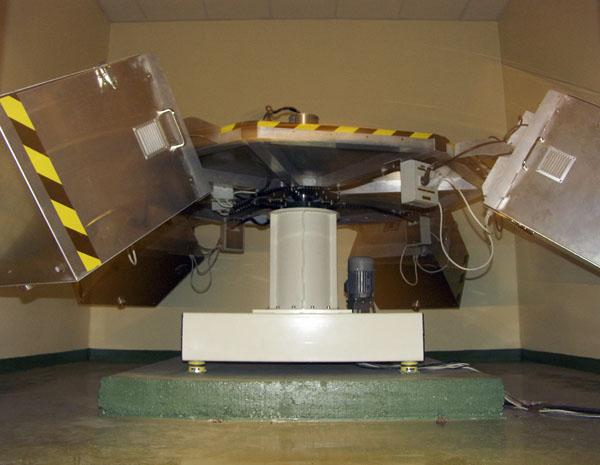
\includegraphics[width=0.7\textwidth]{photo_centrifugeuse.png}
				\caption[Photographie de la centrifugeuse]{Photographie de la centrifugeuse utilisée.}
				\label{photo_centrifugeuse}
			\end{figure}

			\lipsum[2]\index{Nam dui ligula}

\section{Deuxième partie du deuxième chapitre}

	Le faisceau passe ensuite dans un module comprenant un cristal non linéaire permettant de doubler le féquence (excitation de \SIrange{345}{500}{\nano\meter}). Toutes les mesures ont été faites entre \SIlist{400;1200}{\nano\meter} avec un pas de \SI{5}{\nano\meter}.
	
	\lipsum[3]\index{Nulla malesuada}

	\subsection{Première sous-partie de la deuxième partie}

		\lipsum[4]\index{Quisque ullamcorper}

	\subsection[Sous-partie 2]{Deuxième sous-partie de la deuxième partie} % entre [] pour le texte dans la TOC

		Ajout d'une nouvelle entrée d'index de la centrifugeuse\index{centrifugeuse}. Les entrées \gls{+a} \gls{2a} \gls{ca} \gls{Aa} \gls{aa} \gls{alpha} {\NoAutoSpaceBeforeFDP}sont dans la nomenclature. On peux utiliser les commandes personnelles pour appeler rapidement des formules lors de la rédaction \acc et passer des arguments aux commandes pour en modifier l'éxécution \emiss[\nu]{\Omega}.
		
		\subsubsection{Ce titre de partie ne s'affiche pas dans la TOC (tocdepth=2) mais dans la TOC locale (etocsettocdepth=3)}

			Voir (Tableaux~\ref{table:alpha}~et~\ref{table:butcher}).

			\paragraph{Ce titre de partie n'est pas numéroté (secnumdepth=3)}~~\\ % ~~\\ fait le saut de ligne après le titre de 'paragraph' sinon le texte suivant est accolé au titre

				% ce saut de ligne indente le texte de 'paragraph' sinon le paragraphe débute à la marge
				Ajout d'une citation entre parenthèses et tous les auteurs~\parencite{zohdy_mapping_2012}.

			\paragraph{Plusieurs figures côte à côte}~~\\

				\lipsum[66]


				\begin{figure}
					\centering
					\subfloat[Figure A]{\includegraphics[width=.5\textwidth, max height=2in]{example-image-a}}
					\subfloat[Figure B]{\includegraphics[width=.5\textwidth, max height=2in]{example-image-b}}
					\caption{Deux figures}
					\label{fig:deux_figures}
				\end{figure}

			\paragraph{Paramétrer siunitx avec sisetup}~~\\
			
        		Célérité de la lumière dans le vide: $$c=\SI{2.99792458e8}{\meter\per\second}$$


	\chapter{ Résultats}
\chaptertoc{}

\section{Modèles}

	%% tableau nécessitant des filets verticaux
	\begin{table}[h!tbp]
		\begin{center}
			\begin{tabular}{c|*{5}{c}}
			0\\
			$c_2$    & $a_{21}$\\
			$c_3$    & $a_{31}$ & $a_{32}$\\
			$\vdots$ & $\vdots$ &           & $\ddots$\\
			$c_s$    & $a_{s1}$ & $a_{s2}$  & $\cdots$ & $a_{s,s - 1}$\\
			\hline
			         & $b_1$    & $b_2$     & $\cdots$ & $b_{s-1}$     & $b_s$\\
			\end{tabular}
		\end{center}
		\caption{Tableau de Butcher}
		\label{table:butcher}
	\end{table}

	%% tableau avec booktabs (sans filets verticaux)
	\begin{table}[h!tbp]
		\begin{center}
			\begin{tabular}{@{}lcc@{}} \toprule
			$\lambda$ (nm) & $(\alpha_{\lambda}/\alpha_{426,7})_{moy}$ & écart type \\ \midrule
			391,9 \& 392,1 & 0,12 & 0,01 \\
			588,9 \& 589,2 & 0,45 & 0,07 \\
			657,8 \& 658,3 & 6,70 & 0,06 \\
			711,3 & 0,16 & 0,01 \\
			711,6 & 0,15 & 0,01 \\
			712 & 0,31 & 0,02 \\ \bottomrule
			\end{tabular}
		\end{center}
		\caption[Valeur moyenne et écart type des rapports $\alpha_{\lambda}/\alpha_{426,7}$]{Valeur moyenne et écart type des rapports $\alpha_{\lambda}/\alpha_{426,7}$ mesurés pour les chocs plasma de la deuxième série.}
		\label{table:alpha}
	\end{table}

%\newpage

\section{Articles}

	\fullcite{mohamed_clinical_2014}
	% avant d'intégrer un article dans votre thèse, consulter http://www.sherpa.ac.uk/romeo/ si vous souhaitez diffuser sur internet
	\includepdfset{pagecommand=\thispagestyle{scrheadings}} % ajoute la numérotation continue des pages aux fichiers pdf importés
	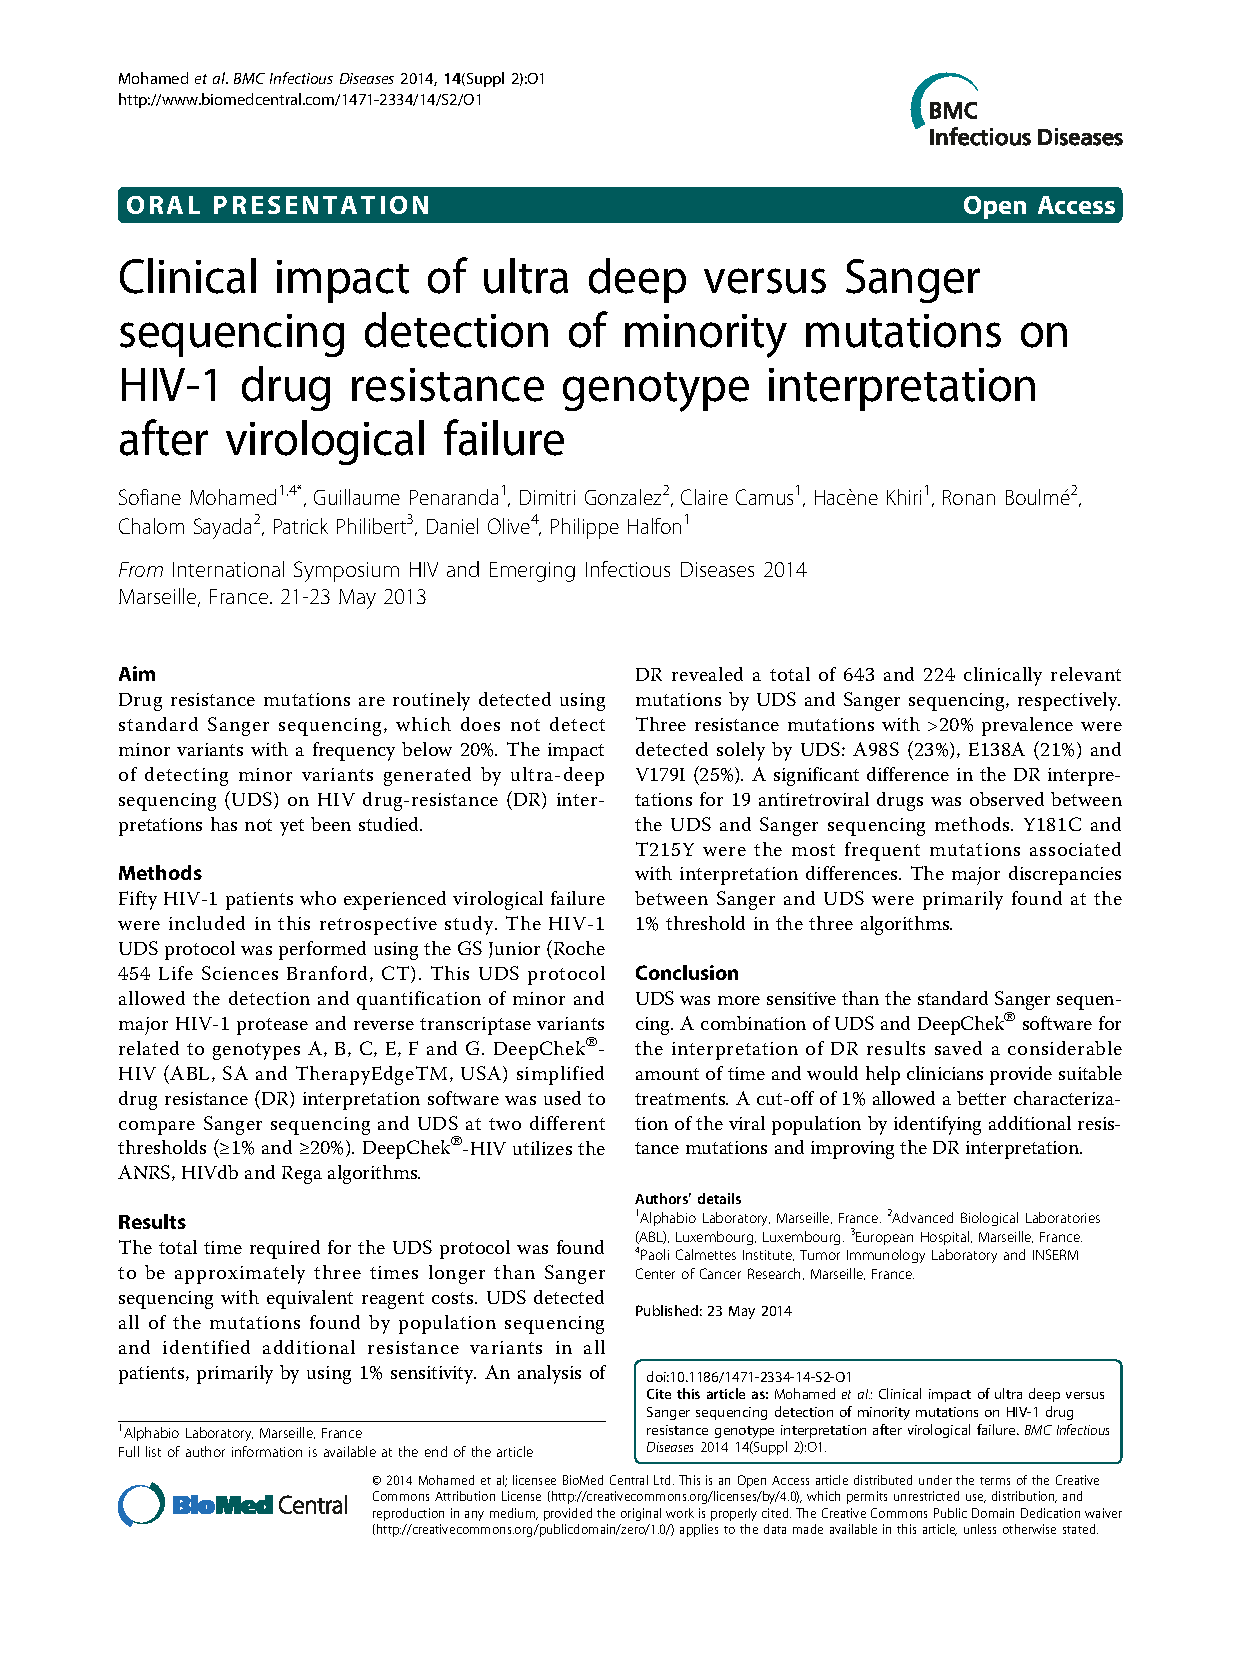
\includepdf[scale=0.9,pages=-]{BMC-1471-2334-14-S2-O1.pdf} % 'scale' ajuste la taille du pdf, vous pouvez affiner en fonction des marges


	%--------------------------------------------------------------------------------------------------
\addchap{Conclusion}
%\addcontentsline{toc}{chapter}{Conclusion}
\label{concs}
Across this thesis we studied explainable deep learning proposals, to understand current image 
recognition models. Explainable Artificial Intelligence and Interpretability are blooming fields 
within the research on machine learning. In particular, current high performing models are 
being steadily assimilated within society and their prominence in human life is increasing. Thus, 
it has become important understanding the processes prompting a prediction in one such model. 
Furthermore, these fields are being studied following a plethora of axis of research. Still, the 
work presented by Lipton \autocite{mythos_interp} and Zhang \autocite{zhang2021survey} lay the 
foundation for our work.\\

\paragraph{Background}
\noindent In Chapter \ref{ch:rel}, we introduced and described the evolution of image recognition 
models. We started with models based on traditional machine learning algorithms, to current high 
performance architectures based attention computation. In relation to this modelling evolution, we 
demonstrated how the improvement of image recognition models consequently benefits the development 
of related Computer Vision fundamental tasks. Thus, further development of image recognition models 
is acknowledged as a major task in Computer Vision, enhancing adjacent tasks within the discipline.\\

\noindent Complementary to the introduction of these models, we highlighted the 
necessity of providing explanations to current image recognition models. We mentioned the proposition  
of the European AI act for regulation of Artificial Intelligence technologies, as well as in the 
Mythos of Model Interpretability by Lipton. In particular, following Lipton's work we 
revised the properties proposed therein, as well as illustrated how they can be adapted to explain 
current state-of-the-art models. Furthermore, we demonstrated our interest on \gls{cam} methods 
to produce explanations. A thorough description of their computation and different proposals is 
established to lay the foundation for the following studies.\\

\noindent Finally, to complement interpretability studies, the background established
evaluation procedures for explainability methods. Regarding these evaluation procedures, we grouped 
them according to the reasoning of the measurement provided, as well as highlighted the positive 
and negative points of each procedure. Notably, Interpretable Object Recognition and 
Causal Analysis are observed to best assess interpertability properties of a model. On one 
hand, it is observed that Interpretable Object Localization implies that model 
interpretations should be aligned to human interpretations. On the other hand, pure human 
measurements are completely aligned with what individuals deem salient on images, which is often 
biased and not often replicable on most experimental settings. Pure classifier centric evaluation 
ultimately addresses these shortcomings, removing implicit bias produced by human reasoning, 
although not from supervision.\\

\paragraph{Opti-CAM}
\noindent Chapter \ref{ch:opticam} presented our first contribution: Opti-CAM, a post-hoc 
interpretability method, constructed following the principles of CAM and evaluation 
procedures. Specifically, Opti-CAM produces a saliency map that maximizes predictive probability 
of images masked by it. Additionally, issues regarding quantitative evaluation are displayed, 
most importantly the incompleteness of Interpretability Object Recognition. To address these 
shortcomings, we proposed Average Gain, a complementary metric to Average Drop, measuring 
the predictive gains obtained while considering explanation maps as input images.\\


\noindent On one hand, we observed that true to its design, Opti-CAM outperforms contemporary 
CAM attribution methods in most quantitative measurements. In particular, this methodology 
performs the best in Interpretable Image Recognition and Causal Analysis, but fails in Object 
Localization. We made sense of these observations aided with visualizations. In contrast to 
current CAM methods, Opti-CAM generates a saliency map that is spread across the input image. 
From this we infer that context matters describing an explanation. Consequently, since context is 
necessary to explain a prediction, the requirement of saliency maps being localized is 
counterintuitive and does not hold.\\

\noindent Lastly, regarding Average Gain our experimental results demonstrated its complementary 
behavior to Interpretable Image Recognition Evaluation.  In particular, this metric efficiently 
demonstrates how Fake-CAM fails as an attribution method: although it attains almost perfect 
Average Drop; its Average Gain measurement fails entirely, effectively complementing the 
shortcomings instated by this CAM method.\\

\paragraph{Cross-Attention Stream}
\noindent Chapter \ref{ch:castream} presented our second contribution, the Cross-Attention Stream. 
This addition inspired by pure attention architectures, computes an abstract representation of 
classes, via interaction of a class token and feature maps across different depths of a model. 
Additionally, this approach was validated in common image recognition models studied on 
interpretability such as ResNet, as well as in a family of models not often studied in this fashion: 
ConvNeXt.\\

\noindent In this contribution we set the stage for quantitative interpretability measurements for 
transparency based approaches. We trained the stream similarly to prior transparency approaches, 
and we evaluated its properties using \gls{cam}, a post-hoc method. Moreover, we observed that our 
saliency maps do not differ much from the baseline ones. However, this result was expected as this 
approach does not modify existing parameters within the network, nor changes the computation of 
attributions. Instead, our representation conveys information differently to the classifier, 
enhancing predicted probability of groundtruth classes. \\

\paragraph{Gradient Denoising}
\noindent Lastly, Chapter \ref{ch:grad} introduced a learning paradigm for interpretable gradients. 
In this approach, the guided backpropagated gradient of the network, observed in the input space is 
used to regularize the network during training, enhancing interpretability properties. Continuing 
with the evaluation of transparency methods seen on Chapter \ref{ch:castream}, we evaluate these 
properties using CAM methods.\\

\noindent Notably, the learning paradigm was showcased in a constrained setting: small datasets and 
low parameter networks. This setting is a consequence of the computational cost this approach 
requires. However, the results obtained in this manner are promising, therefore addressing the 
prior complexity would allow for scaling on to large scale image datasets and more complex models. 
This ultimately is one direction this idea can be expanded on in the future. 

	\appendix

	\newpage
	\printbibliography[heading=bibintoc]%% bibliographie
	
	\newpage
	\printindex							%% index
	
	\newpage
	\printendnotes						%% notes

	\setcounter{chapter}{0}
\renewcommand{\thesection}{\Alph{section}}

\chapter*{ANNEXES}
\newpage
\addcontentsline{toc}{chapter}{ANNEXES}

\section{Intitulés des doctorats AMU}
\label{chap:doctorats}

		\begin{itemize}
		\item Discipline
			\begin{itemize}
			\item Spécialité
			\end{itemize}
		\end{itemize}
		
	\subsection*{ED 62 SCIENCES DE LA VIE ET DE LA SANTE}\label{ed-62-sciences-de-la-vie-et-de-la-sante}

		\begin{itemize}
		\item Biologie santé
			\begin{itemize}
			\item Biochimie structurale
			\item Génomique et  Bioinformatique
			\item Biologie du développement
			\item Immunologie
			\item Génétique
			\item Microbiologie
			\item Biologie végétale
			\item Neurosciences
			\item Oncologie
			\item Maladies infectieuses
			\item Pathologie vasculaire et nutrition
			\item Ethique
			\item Recherche clinique et Santé Publique
			\item Biotechnologie
			\end{itemize}
		\end{itemize}

	\subsection*{ED 67 SCIENCES JURIDIQUES ET POLITIQUES}\label{ed-67-sciences-juridiques-et-politiques}

		\begin{itemize}
		\item Droit
			\begin{itemize}
			\item Droit Privé
			\item Droit Public
			\item Histoire du Droit
			\end{itemize}
		\item Science Politique
		\end{itemize}

	\subsection*{ED 184 MATHEMATIQUES ET INFORMATIQUE}\label{ed-184-mathematiques-et-informatique}

		\begin{itemize}
		\item Mathématiques
		\item Informatique
		\item Automatique
		\end{itemize}

	\subsection*{ED 250 SCIENCES CHIMIQUES DE MARSEILLE}\label{ed-250-sciences-chimiques-de-marseille}

		\begin{itemize}
		\item Sciences Chimiques
		\end{itemize}

	\subsection*{ED 251 SCIENCES DE L'ENVIRONNEMENT}\label{ed-251-sciences-de-lenvironnement}

		\begin{itemize}
		\item Sciences de l'Environnement
			\begin{itemize}
			\item Anthropologie biologique
			\item Ecologie
			\item Géosciences 
			\item Génie des procédés
			\item Océanographie
			\item Chimie 
			\item Environnement et santé 
			\end{itemize}
		\end{itemize}

	\subsection*{ED 352 PHYSIQUE ET SCIENCES DE LA MATIERE}\label{ed-352-physique-et-sciences-de-la-matiere}

		\begin{itemize}
		\item Physique et Sciences de la Matière 
			\begin{itemize}
			\item Astrophysique et Cosmologie
			\item Biophysique
			\item Energie, Rayonnement et Plasma
			\item Instrumentation
			\item Optique, Photonique et Traitement d'Image
			\item Physique des Particules et Astroparticules
			\item Physique Théorique et Mathématique
			\item Matière Condensée et Nanosciences 
			\end{itemize}
		\end{itemize}

	\subsection*{ED 353 SCIENCES POUR L'INGENIEUR: MECANIQUE, PHYSIQUE, MICRO ET NANOELECTRONIQUE}\label{ed-353-sciences-pour-lingenieur-mecanique-physique-micro-et-nanoelectronique}

		\begin{itemize}
		\item Sciences pour l'Ingénieur
			\begin{itemize}
			\item Energétique
			\item Mécanique et physique des fluides 
			\item Acoustique
			\item Mécanique des solides
			\item Micro et Nanoélectronique
			\item Génie civil et architecture
			\item Nucléaire de fission 
			\item Fusion magnétique
			\end{itemize}
		\end{itemize}

	\subsection*{ED 354 LANGUES, LETTRES ET ARTS}\label{ed-354-langues-lettres-et-arts}

		\begin{itemize}
		\item Etudes anglophones
		\item Etudes germaniques
		\item Etudes slaves
		\item Langues et littératures d'Asie
			\begin{itemize}
			\item Chinois
			\item Vietnamien
			\item Coréen
			\end{itemize}
        	\item Arts
            		\begin{itemize}
            		\item Arts plastiques 
            		\item Sciences de l'art
            		\item Musique et musicologie
            		\item Etudes cinématographiques et audiovisuelles
            		\item Arts de la scène
            		\item Médiation culturelle des arts
            		\end{itemize}
        	\item Pratique et théorie de la création artistique et littéraire
		\item Langue et Littératures françaises
		\item Littérature générale et comparée
		\item Langues, littératures et civilisations romanes 
			\begin{itemize}
			\item Etudes hispaniques et latino-américaines
			\item Etudes italiennes
			\item Etudes roumaines
			\end{itemize}
		\end{itemize}

	\subsection*{ED 355 ESPACES, CULTURES, SOCIETES}\label{ed-355-espaces-cultures-societes}

		\begin{itemize}
		\item Géographie
		\item Démographie
		\item Urbanisme et Aménagement du territoire
		\item Préhistoire
		\item Archéologie
		\item Histoire de l'Art
		\item Histoire
		\item Sciences de l'Antiquité
		\item Mondes arabe, musulman et sémitique
		\item Etudes romanes
		\item Sociologie
		\item Anthropologie
		\item Architecture
		\item Cultures et Sociétés d'Asie
		\end{itemize}

	\subsection*{ED 356 COGNITION, LANGAGE, EDUCATION}\label{ed-356-cognition-langage-education}

		\begin{itemize}
		\item Philosophie
		\item Psychologie
		\item Sciences du Langage
		\item Sciences de l'Information et de la Communication
		\item Sciences de l'Education
		\item Sciences Cognitives
		\end{itemize}

	\subsection*{ED 372 SCIENCES ECONOMIQUES ET DE GESTION}\label{ed-372-sciences-economiques-et-de-gestion}

		\begin{itemize}
		\item Sciences de Gestion
		\item Sciences Economiques
		\end{itemize}

	\subsection*{ED 463 SCIENCES DU MOUVEMENT HUMAIN}\label{ed-463-sciences-du-mouvement-humain}

		\begin{itemize}
		\item Sciences du Mouvement Humain 
		\end{itemize}


\newpage
\section{Données brutes}

	\lipsum[1-4]
			%% annexes

\end{document}
